\section{Experiments}
\label{sec:sqair_experiments}

We evaluate \gls{SQAIR} on two datasets.
Firstly, we perform an extensive evaluation on moving \gls{MNIST} digits, where we show that it can learn to reliably detect, track and generate moving digits (\Cref{sec:expr_mnist}). Moreover, we show that \gls{SQAIR} can simulate moving objects into the future --- an outcome it has not been trained for. 
We also study the utility of learned representations for a downstream task.
Secondly, we apply \gls{SQAIR} to real-world pedestrian CCTV data from static cameras (\textit{DukeMTMC}, \cite{Ristani2016performance}), where we perform background subtraction as pre-processing. In this experiment, we show that \gls{SQAIR} learns to detect, track, predict and generate walking pedestrians without human supervision.

\subsection{Moving multi-\textsc{mnist}}
\label{sec:expr_mnist}

\begin{figure}
    \centering
    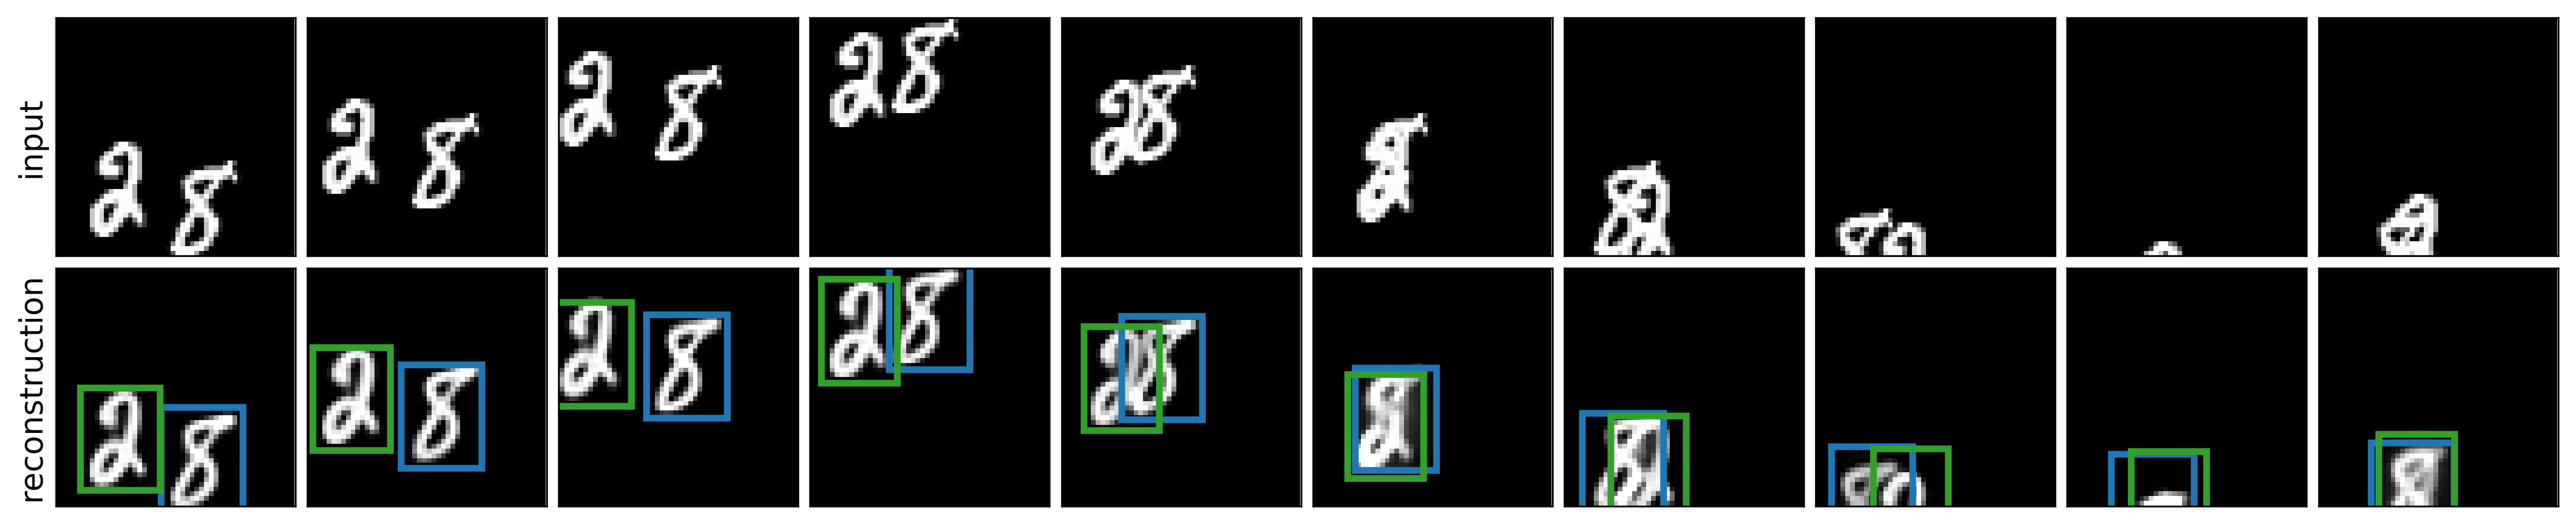
\includegraphics[width=\linewidth]{figures/SQAIR/mnist_rec/000106}
    \caption{Input images (top) and \gls{SQAIR} reconstructions with marked glimpse locations (bottom). For more examples, see \Cref{fig:mnist_recs_additional} in \Cref{app:mnist_visual}.}
    \label{fig:mnist_recs}
\end{figure}

\begin{figure}
    \centering
    
\includegraphics[width=\linewidth]{figures/SQAIR/mnist_samples/000102}
    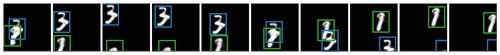
\includegraphics[width=\linewidth]{figures/SQAIR/mnist_samples/000078}
    \caption{Samples from \gls{SQAIR}. Both motion and appearance are consistent through time, thanks to the propagation part of the model. For more examples, see \Cref{fig:mnist_samples_additional} in \Cref{app:mnist_visual}.}
    \label{fig:mnist_samples}
\end{figure}
\begin{figure}
    \centering
    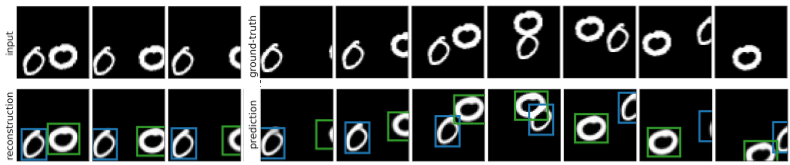
\includegraphics[width=\linewidth]{figures/SQAIR/sqair_mnist_conditional_after_three}
    \caption{The first three frames are input to \gls{SQAIR}, which generated  the rest conditional on the first frames.}
    \label{fig:mnist_cond_gen}
\end{figure}

\begin{figure}
    \centering
    \begin{minipage}[c]{0.3\linewidth}
        \centering
        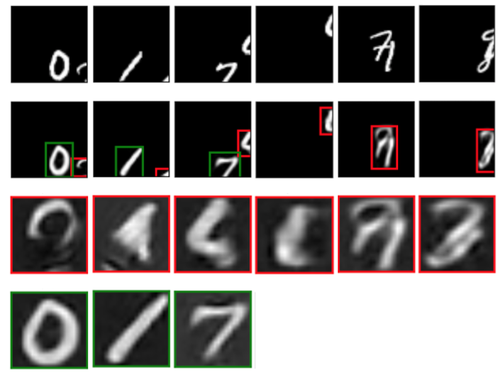
\includegraphics[width=\linewidth]{figures/SQAIR/air_partial_glimpse}
    \end{minipage}
    \hfill
    \begin{minipage}[c]{0.3\linewidth}
        \centering
        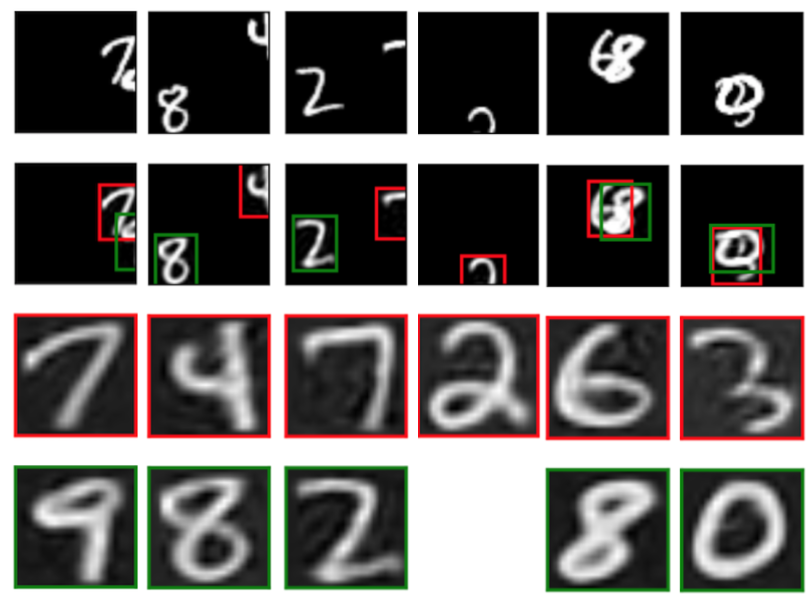
\includegraphics[width=\linewidth]{figures/SQAIR/sqair_partial_glimpse}
    \end{minipage}
       \hfill
    \begin{minipage}[c]{0.35\linewidth}
        \centering
        \caption{Inputs, reconstructions with marked glimpse locations and reconstructed glimpses for \gls{AIR} (left) and \gls{SQAIR} (right). \Gls{SQAIR} can model partially visible and heavily overlapping objects by aggregating temporal information.}
        \label{fig:partial_glimpse}
    \end{minipage}
\end{figure}


The dataset consists of sequences of length 10 of multiple moving \gls{MNIST} digits. All images are of size $50 \times 50$ and there are zero, one or two digits in every frame (with equal probability).
Sequences are generated such that no objects overlap in the first frame, and all objects are present through the sequence; the digits can move out of the frame, but always come back.
See \Cref{app:mnist_inout} for an experiment on a harder version of this dataset.
There are 60,000 training and 10,000 testing sequences created from the respective \gls{MNIST} datasets.
We train two variants of \gls{SQAIR}: the \textsc{mlp}-\gls{SQAIR} uses only fully-connected networks, while the \textsc{conv}-\gls{SQAIR} replaces the networks used to encode images and glimpses with convolutional ones; it also uses a subpixel-convolution network as the glimpse decoder \citep{Shi2016subpixel}.
See \Cref{app:mnist_details} for details of the model architectures and the training procedure.

We use \gls{AIR} and \gls{VRNN} \citep{Chung2015} as baselines for comparison.  \gls{VRNN} can be thought of as a sequential \gls{VAE} with an \gls{RNN} as its deterministic backbone. Being similar to a \gls{VAE}, its latent variables are not structured, nor easily interpretable. For a fair comparison, we control the latent dimensionality of $\gls{VRNN}$ and the number of learnable parameters. We provide implementation details in \Cref{apd:vrnn}.

\begin{table}
    \centering
    \begin{tabular}{c|c|c|c|c|c}
                         & $\log \p{\bxTs}{}{\theta}$ & $\log \p{\bxTs}{\bzTs}{\theta}$  & $\kl{\q{}{}{\phi}}{\p{}{}{\theta}}$ & Counting & Addition\\
                         \hline
        \textsc{conv}-\gls{SQAIR} & $\bm{6784.8}$ & $\bm{6923.8}$ & $\bm{134.6}$ & $0.9974$ & $0.9990$ \\
        \textsc{mlp}-\gls{SQAIR}  & $6617.6$      & $6786.5$      & $164.5$      & $\mathbf{0.9986}$ & $\mathbf{0.9998}$ \\
        \textsc{mlp}-\gls{AIR}    & $6443.6$      & $6830.6$      & $352.6$      & $0.9058$ & $0.8644$\\
        \textsc{conv}-\gls{VRNN}  & $6561.9$      & $6737.8$      & $270.2$      & n/a & $0.8536$\\
        \textsc{mlp}-\gls{VRNN}   & $5959.3$      & $6108.7$      & $218.3$      & n/a  & 0.8059 \\
    \end{tabular}
    \vspace{5pt}
    \caption{\gls{SQAIR} achieves higher performance than the baselines across a range of metrics. The third column refers to the \gls{KL} divergence between the approximate posterior and the prior. Counting refers to accuracy of the inferred number of objects present in the scene, while addition stands for the accuracy of a supervised digit addition experiment, where a classifier is trained on the learned latent representations of each frame.}
    \label{tab:quant}
\end{table}

The quantitative analysis consists of comparing all models in terms of the marginal log-likelihood $\log \p{\bxTs}{}{\theta}$ evaluated as the $\loss[\textsc{IWAE}]$ bound with $K=1000$ particles, reconstruction quality evaluated as a single-sample approximation of $\expc[\q{}{}{\phi}]{\log \p{\bxTs}{\bzTs}{\theta}}$ and the \gls{KL}-divergence between the approximate posterior and the prior (\Cref{tab:quant}). Additionally, we measure the accuracy of the number of objects modelled by \gls{SQAIR} and \gls{AIR}. \Gls{SQAIR} achieves superior performance across a range of metrics --- its convolutional variant outperforms both \gls{AIR} and the corresponding \gls{VRNN} in terms of model evidence and reconstruction performance. 
The \gls{KL} divergence for \gls{SQAIR} is almost twice as low as for \gls{VRNN} and by a yet larger factor for \gls{AIR}.
We can interpret \gls{KL} values as an indicator of the ability to compress, and we can treat \gls{SQAIR}/\gls{AIR} type of scheme as a version of run-length encoding.
While \gls{VRNN} has to use information to explicitly describe every part of the image, even if some parts are empty, \gls{SQAIR} can explicitly allocate content information ($\bz^\mathrm{what}$) to specific parts of the image (indicated by $\bz^\mathrm{where}$).
\Gls{AIR} exhibits the highest values of \gls{KL}, but this is due to encoding every frame of the sequence independently --- its prior cannot take \textit{what} and \textit{where} at the previous time-step into account, hence higher KL.
The fifth column of \Cref{tab:quant} details the object counting accuracy, that is indicative of the quality of the approximate posterior. It is measured as the sum of $\zt^\mathrm{pres}$ for a given frame against the true number of objects in that frame. As there is no $z^\mathrm{pres}$ for \gls{VRNN} no score is provided. Perhaps surprisingly, this metric is much higher for \gls{SQAIR} than for \gls{AIR}. This is because \gls{AIR} mistakenly infers overlapping objects as a single object. Since \gls{SQAIR} can incorporate temporal information, it does not exhibit this failure mode (\textit{cf}. \Cref{fig:partial_glimpse}).
Next, we gauge the utility of the learnt representations by using them to determine the sum of the digits present in the image (\Cref{tab:quant}, column six). To do so, we train a 19-way classifier (mapping from any combination of up to two digits in the range $[0, 9]$ to their sum) on the extracted representations and use the summed labels of digits present in the frame as the target. \Cref{app:mnist_details} contains details of the experiment. 
\Gls{SQAIR} significantly outperforms \gls{AIR} and both variants of \gls{VRNN} on this tasks.
\Gls{VRNN} under-performs due to the inability of disentangling overlapping objects, while both \gls{VRNN} and \gls{AIR} suffer from low temporal consistency of learned representations, see \Cref{app:mnist_visual}. 
Finally, we evaluate \gls{SQAIR} qualitatively by analyzing reconstructions and samples produced by the model against reconstructions and samples from \gls{VRNN}.
We observe that samples and reconstructions from \gls{SQAIR} are of better quality and, unlike \gls{VRNN}, preserve motion and appearance consistently through time. See \Cref{app:mnist_visual} for direct comparison and additional examples.
Furthermore, we examine conditional generation, where we look at samples from the generative model of \gls{SQAIR} conditioned on three images from a real sequence (see \Cref{fig:mnist_cond_gen}).
We see that the model can preserve appearance over time, and that the simulated objects follow similar trajectories, which hints at good learning of the motion model (see \Cref{app:mnist_visual} for more examples).
\Cref{fig:partial_glimpse} shows reconstructions and corresponding glimpses of \gls{AIR} and \gls{SQAIR}. Unlike \gls{SQAIR}, \gls{AIR} is unable to recognize objects from partial observations, nor can it distinguish strongly overlapping objects (it treats them as a single object; columns five and six in the figure).
We analyze failure cases of \gls{SQAIR} in \Cref{app:fail}.



\subsection{Generative Modelling of Walking Pedestrians}
\label{sec:expr_duke}

\begin{figure}
    \centering
    \begin{minipage}[c]{0.49\linewidth}
        \centering
        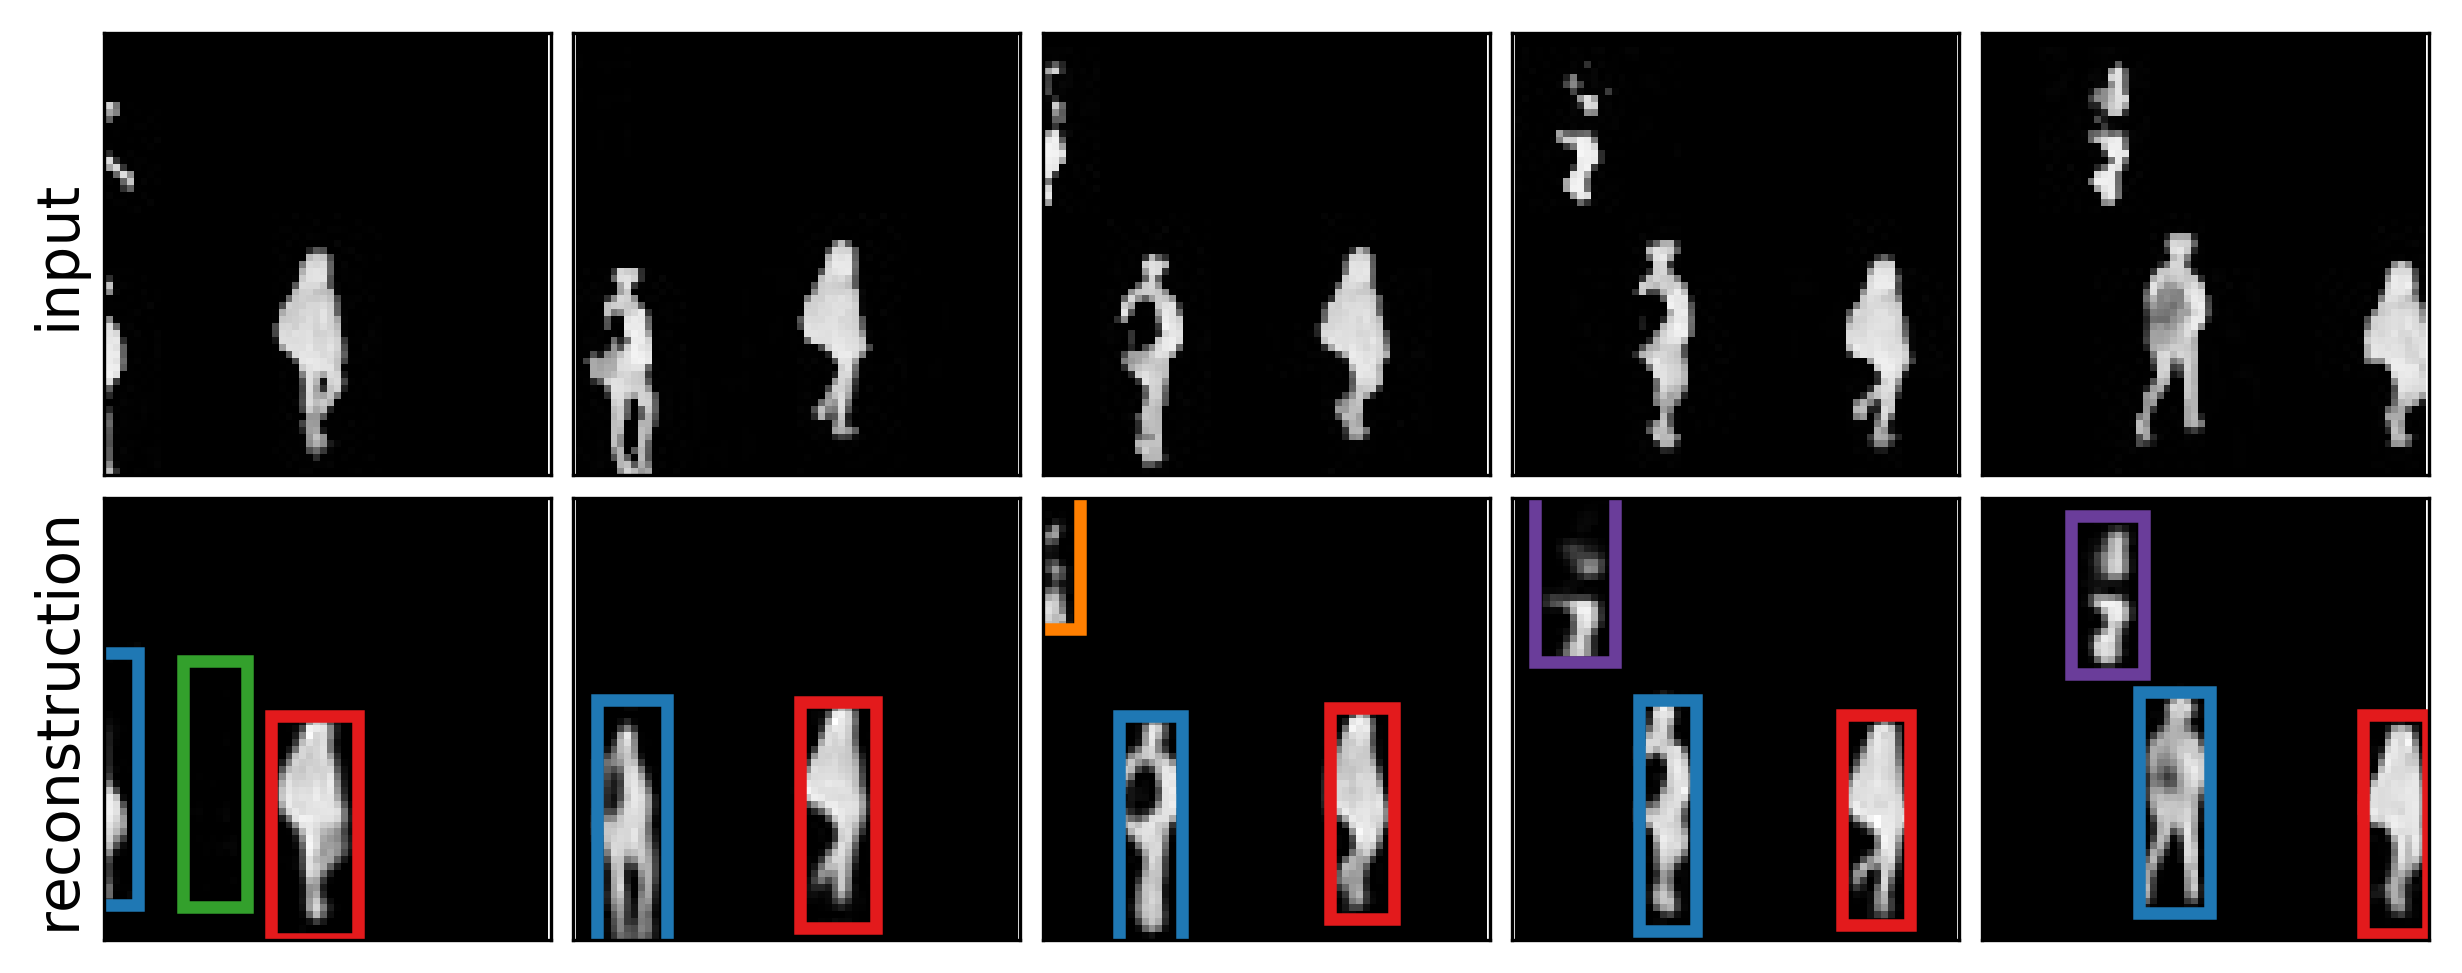
\includegraphics[width=\linewidth]{figures/SQAIR/duke_rec/front/000065}
        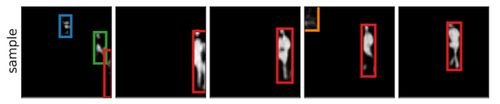
\includegraphics[width=\linewidth]{figures/SQAIR/duke_sample/front/sqair_duke_sample_with_label_296}
    \end{minipage}
    \hfill
    \begin{minipage}[c]{0.49\linewidth}
        \centering
        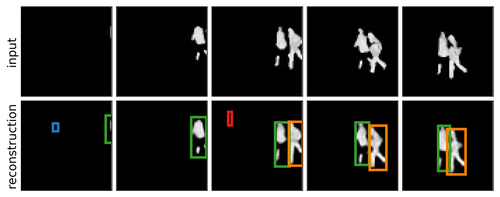
\includegraphics[width=\linewidth]{figures/SQAIR/duke_rec/front/000099}
       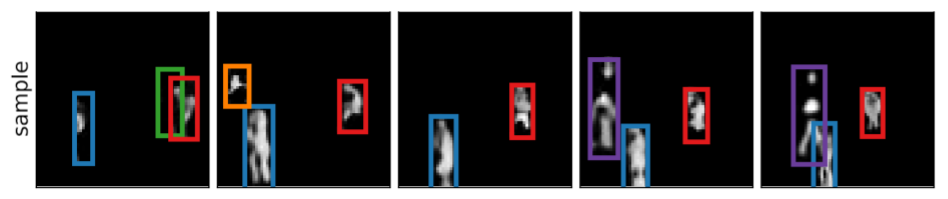
\includegraphics[width=\linewidth]{figures/SQAIR/duke_sample/front/sqair_duke_sample_with_label_020}
    \end{minipage}
    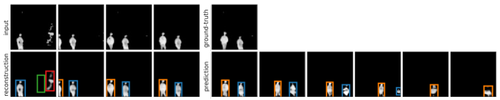
\includegraphics[width=.95\linewidth]{figures/SQAIR/duke_cond_gen/front/sqair_duke_cond_after_four}
    \caption{Inputs on the top, reconstructions in the second row, samples in the third row; rows four and five contain inputs and conditional generation: the first four frames in the last row are reconstructions, while the remaining ones are predicted by sampling from the prior. There is no ground-truth, since we used sequences of length five of training and validation.}
    \label{fig:duke_rec}
\end{figure}
To evaluate the model in a more challenging, real-world setting, we turn to data from static CCTV cameras of the \textit{DukeMTMC} dataset \citep{Ristani2016performance}. As part of pre-precessing, we use standard background subtraction algorithms \citep{Itseez2015opencv}. In this experiment, we use $3150$ training and $350$ validation sequences of length $5$. For details of model architectures, training and data pre-processing, see \Cref{app:duke_details}.
We evaluate the model qualitatively by examining reconstructions, conditional samples (conditioned on the first four frames) and samples from the prior (\Cref{fig:duke_rec} and \Cref{app:duke_visual}).
We see that the model learns to reliably detect and track walking pedestrians, even when they are close to each other.

There are some spurious detections and re-detections of the same objects, which is mostly caused by imperfections of the background subtraction pipeline --- backgrounds are often noisy and there are sudden appearance changes when a part of a person is treated as background in the pre-processing pipeline.
The object counting accuracy in this experiment is $0.5712$ on the validation dataset, and we noticed that it does increase with the size of the training set. We also had to use early stopping to prevent overfitting, and the model was trained for only $315$k iterations ($>1$M for \textsc{mnist} experiments). Hence, we conjecture that accuracy and marginal likelihood can be further improved by using a bigger dataset.